\chapter{Consistency through different transcriptomics studies with RNA-Seq}
\label{ch:Transcriptomics}



Science progresses through many elements. Quantified observations are rather one
of the fastest tracks to new understandings and insights.

\section{Introduction}

\begin{itemize}
    \item Difficulty of sampling of normal conditions for human, particularly
        for the solid tissues. (could be very useful in case of cancer for
        example)
    \item Lots of transcriptomics data in the repository of \EBI{}. Can we use
        this as a base for reference? + Explosion of atlases publications
    \item previous point not new, but recently multiplications of studies on
        normal human studies based on \Rnaseq
    \item Indeed, in the past people tried with microarray data but didn't work
        \TK{find sources}
    \item When I started this study, there wasn't any publication on this matter
        yet, but \Rnaseq was considered as quantitative (when microarrays were
        considered semi-quantitative at best).
    \item nobody did published on my specific subject yet, but since then things changed
    \item first paper from MACQ/SEC III
    \item increasing number of papers that been published on the subject
    \item I will discuss the different part of the papers that are relevant
        with additions on what my study confirms/refutes or expands them.
\end{itemize}
\section{EBI Expression Atlas or how integrating independent datasets }

While current high-throughput gene expression studies are mainly about
differential gene expression between (notably diseased and treated) conditions,
healthy controls are not always enough or even available. Even more so, when the
study subject is human. Indeed, it rather apprehensible that sampling solid
tissues on a healthy human is (Fortunately) not usual or common.

Although, many atlases have been released to help on this issue,
there is still not any direct method that would allow you more than check the
presence (or lack of detection) of specific genes in a given condition.

With the increasing number of studies of normal tissues with overlapping conditions
\cref{fig:VennStudiesT}, we are investigating the consistency of gene-tissue
associations on one side but moreover we would like to assess the expression
levels across the datasets in the aim of integrating all the available data in a
gene expression baseline reference.

When I started this project no study (either comprehensive or not) was
investigating in-depth the consistency of transcriptome expression measurements.
However, in August 2014 a paper comparing different preparation methods,
sequencing technologies operated in different laboratories
on samples from the same biological source concludes that while absolute
measurements are not consistent, the relative expression is highly consistent
(95\% Pearson correlation?)

\begin{comment}
The main question when I started this project was to appraise how much consistent
(robust) is the \Rnaseq\ technology to quantify the gene expression. While it
is comparable to microarrays for differential gene expression analysis study
\TK{add reference},
\Rnaseq\ plus: detect new things - minus: sampling problems (stuff might be there
but won't be ``fished''.
\end{comment}

When I started this work in 2013, there were only three complying
datasets at that time. Fortunately, I was later
able to incorporate two other datasets to my study. One of them is the \Gtex\
(v4) data and the other one is the Uhlén et al.\ dataset (first
published as \citet{Uhlen2014} and then extended for the \citet{Uhlen2015} publication).
The number of provided samples and covered tissues for these two datasets
is far greater than the other ones. These \dataset{\Gtex} and \dataset{Uhlén}
datasets are indeed presenting a greater set of common tissues. Moreover,
the more recent and similar technology used (either for the libraries preparation,
the sequencer or the paired-end protocols) and the studies design that includes
biological replicates for every tissue had motivated a more focused comparison
based only on these two datasets.

\begin{comment}
While I downloaded and entirely processed four of the transcriptomic datasets
myself, it was not the case for the \Gtex\ dataset. Since this
data is involved in many project within the \EBI\ and due to its huge amount of
data, it was agreed that this would be processed centrally by one person and then
redistributed to all the other interested parties. Dr Nuno Fonseca had this
tremendous task and provided me with quantification data,
both for each sample separately and then for each tissue (all relevant samples
pooled together).

For the sake of consistency, that led me to reprocess all the other four datasets
to comply with the reference used for the \Gtex\ samples. The silver lining
was that they were built with the new reference of the
Human genome GRCH 38 (ENSEMBL v. 76).
\end{comment}


With each version of annotation and addition of new data,
the results presented in this work got more refined. Nevertheless, the general
trends of the outcomes remained consistent which supports the robustness of the
methodology and the presented conclusions.


\begin{figure}%[!htbp]
    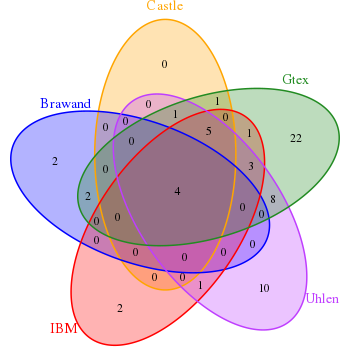
\includegraphics[scale=0.6]{transcriptomics/VennStudiesT}\centering
    \caption[Distribution of unique and shared tissues between the
    transcriptomic datasets]
    {\label{fig:VennStudiesT}\textbf{Distribution of unique and shared tissues
    between the transcriptomic datasets.} The 5 datasets share 4
    common tissues: \tissue{Heart}, \tissue{Kidney}, \tissue{Liver} and
    \tissue{Testis}. The biggest overlap of tissues (23) is between Uhlén et \Gtex.
    These two sets of tissues are the focus of the current study.}
\end{figure}

\Cref{fig:VennStudiesT} presents the five datasets overlapping tissues. We notice
that they all share at least four tissues: \tissue{Heart}, \tissue{Kidney},
\tissue{Liver} and \tissue{Testis}.

We also observe the great number of shared tissues between the two most recent
datasets: \dataset{Uhlen} and \dataset{GTEx}. Indeed, they share together twenty-three
tissues: \tissue{Adipose}, \tissue{Adrenal}, \tissue{Bladder},
\tissue{Cerebral cortex}, \tissue{Colon}, \tissue{Oesophagus},
\tissue{Fallopian tube}, \tissue{Heart}, \tissue{Kidney}, \tissue{Liver},
\tissue{Lung}, \tissue{Ovary}, \tissue{Pancreas}, \tissue{Prostate},
\tissue{Salivary gland}, \tissue{Skeletal muscle}, \tissue{Skin},
\tissue{Small intestine}, \tissue{Spleen}, \tissue{Stomach}, \tissue{Testis},
\tissue{Thyroid} and \tissue{Uterus}.

As we can see in the \cref{tab:Trans5DF}, many of the transcriptomic datasets I
use have been produced through
polyA-selected library protocols, notably the \dataset{Uhlén} dataset which is
used in both study parts.
To avoid as many artefacts as possible, I
focus my study on the \mRNAs\ pool: most of the analyses are excluding
any gene that the biotype is not annotated as \emph{protein coding}.


\section{Results}\label{sec:Trans_Results}

\subsection{Reproducibility of expression profile at tissue level}\label{subsec:Trans_ReproExpresTissue}


\subsection{Tissue specific,housekeeping genes and other categories}\label{subsec:Trans_TissueSpeAndHK}

\subsection{Curated sets}\label{subsec:Trans_curatedSets}


RNA-seq is consistent across datasets; samples are more likely to cluster by
biological origins than by studies. (Figure 2)
While Pearson correlations are higher, without any a priori Spearman correlations
allow a better separation of the different tissues in distinct clusters across
datasets.

Many genes have a consistent profile of expression levels through the different
datasets.
To help EBI Expression Atlas has developed a feature that allows the visualisation
of the expression of a gene (or protein) across the different dataset that it
integrates. (Figure 3)

Reuse of data allows the assessment of the biological quality of a sample.
While RNA-seq workflows integrate numerous quality checks for their different steps,
it is not always easy to appraise the original quality of the samples. Comparing
similar conditions from different sources allow some high level biological check.
Indeed, we noticed that some tissues have a more unique profile in specific
datasets.

Overall gene expressions for protein coding genes across different tissues
correlated highly between datasets. (See part 3. Integration of Transcriptomics
and Proteomics studies – Figure 15)




\section{Discussion}\label{sec:Trans_discussion}



\begin{comment}
  \begin{figure}%[!htbp]
      \includegraphics%[scale=0.6]%
      {transcriptomics/}\centering
      \caption[]
      {\label{fig:}\textbf{}}
  \end{figure}
\end{comment}
